\documentclass[a4paper,10pt]{report}

\topmargin -2cm
%\topskip0cm
%\footskip0cm
%\headsep0cm
\parindent0cm
\oddsidemargin -1cm
\evensidemargin -1cm
\headheight 2cm
\textheight 24cm
\textwidth 18cm

\author{Daniel W\"aber (4049590)}
\title{\"Ubung}

\usepackage{ucs}
\usepackage[utf8x]{inputenc}
\usepackage{german}
\usepackage{color}
\usepackage{url}
\usepackage{graphicx}
\usepackage{algorithmic}

\pagestyle{empty}
\usepackage{makeidx}
\usepackage{amsmath}
\usepackage{amsfonts}
\usepackage{amssymb,euscript}
\usepackage{dsfont}
\usepackage{listings}
\usepackage{enumerate}
\newfont{\Fr}{eufm10}
\newfont{\Sc}{eusm10}
\newfont{\Bb}{msbm10}
\newcommand{\limin}{\lim_{n\rightarrow\infty}}
\newcommand{\limix}{\lim_{x\rightarrow\infty}}
\newcommand{\limun}{\lim_{n\rightarrow -\infty}}
\newcommand{\limux}{\lim_{n\rightarrow -\infty}}
\newcommand{\limx}{\lim_{x\rightarrow x_0}}
\newcommand{\limh}{\lim_{h\rightarrow 0}}
\newcommand{\defi}{\paragraph{Definition:}}
\newcommand{\bew}{\paragraph{Beweis:}}
\newcommand{\satz}{\paragraph{Satz:}}
\newcommand{\bsp}{\paragraph{Beispiel:}}
\newcommand{\lemma}{\paragraph{Lemma:}}
\newcommand{\N}{\mathds{N}}
\newcommand{\F}{\mathds{F}}
\newcommand{\Z}{\mathds{Z}}
\newcommand{\Q}{\mathds{Q}}
\newcommand{\R}{\mathds{R}}
\newcommand{\G}{\mathds{G}}
\newcommand{\C}{\mathds{C}}
\newcommand{\K}{\mathds{K}}
\newcommand{\A}{\mathds{A}}
\newcommand{\E}{\mathcal{E}}
\renewcommand{\P}{\mathcal{P}}
\newcommand{\sigA}{$\sigma$-Algebra }
\newcommand{\qed}{$\hfill\blacksquare$}
\newcommand{\arsinh}{\operatorname{arsinh} }
\newcommand{\arcosh}{\operatorname{arcosh} }
\newcommand{\gdw}{ $ \Leftrightarrow $ }
\newcommand{\tf}{ $ \Rightarrow $ }
\newcommand{\mgdw}{\Leftrightarrow}
\newcommand{\mtf}{\Rightarrow}
\newcommand{\Bild}{\text{Bild}}
\newcommand{\Kern}{\text{kern}}
\newcommand{\rg}{\text{rg}}
\newcommand{\deff}{\text{deff}}

\newcommand{\alphato}{\underset{\alpha}\to}
\newcommand{\betato}{\underset{\beta}\to}
\newcommand{\etato}{\underset{\eta}\to}
\newcommand{\ito}{\underset{i}\to}
\newcommand{\sto}{\underset{s}\to}
\newcommand{\kto}{\underset{k}\to}
\newcommand{\xto}{\underset{x}\to}

\usepackage{fancyhdr}
\pagestyle{fancy}
\lhead{Daniel Waeber\\Alex Muenn}
\chead{"Ubungsblatt \nr\\\today}
\rhead{Bildverarbeitung}



\newcommand{\nr}{1}

\begin{document}
\section*{Aufgaben 1 - Hadamard}
Wie in der Vorlesung beschrieben, wird die Hadamard-Matrix rekursiv generiert:

\lstset{language=matlab}
\begin{lstlisting}[]
function matrix = hadamard(dim)
    if dim <= 1
        matrix = [1];
    else
        if mod(dim,2) != 0
            printf ('unsupported dimension\n');
        else
            m=hadamard(dim/2);
            matrix=[m,m;m,-m];
        end
    end
end
\end{lstlisting}

Die Transformation und R\"ucktransformation lassen sich dann in wenigen Schritten realisieren:


\lstset{language=matlab}
\begin{lstlisting}[]
H = hadamard(rows);
# normieren
H = H/sqrt(rows);

I_trans = H*double(I_in)*H;
I_trans = reduce(I_trans,0.2);
I_out = H*I_trans*H;
\end{lstlisting}

\section*{Aufgabe 2 - Fourier} 

\begin{itemize}
\item Generierung der Fourier-Matrix (complexe Matrix mit I-Teil)
\item bauen von $F^{-1} = F^*$ durch conjugate flip Eigenschaft, up-down-flip von der zweiten bis zur letzten Zeile
\item einfache Berechnung: $I_{trans} = F * I_{in} * F$
\item setzen der ZEROS f\"ur Part III anhand der $abs(I_{trans})$
\item sowie $I_{re} = real( F^* * I_{trans} * F^* )$
\end{itemize}

\section*{Aufgabe 3 - Verlust}
\paragraph{Hadamard}
Es ist m\"oglich den \"uberwiegenden Teil der Elemente in der transformierten 
Matrix zu entfernen, ohne sichtbare Unterschiede zu bemerken. Ab einem gewissen
Punkt jedoch, setzt Rauschen ein, der sich zunehmend verst\"arkt. Die Differenz
zwischen Original und Rekonstruktion zeigt, das Verluste prim\"ar an Frequenz\"uberg\"angen
entstehen. Im abgebildeten Beispiel wurden 254054 der 262144 Elemente in der transformierten
Matrix auf $0$ gesetzt.
\\
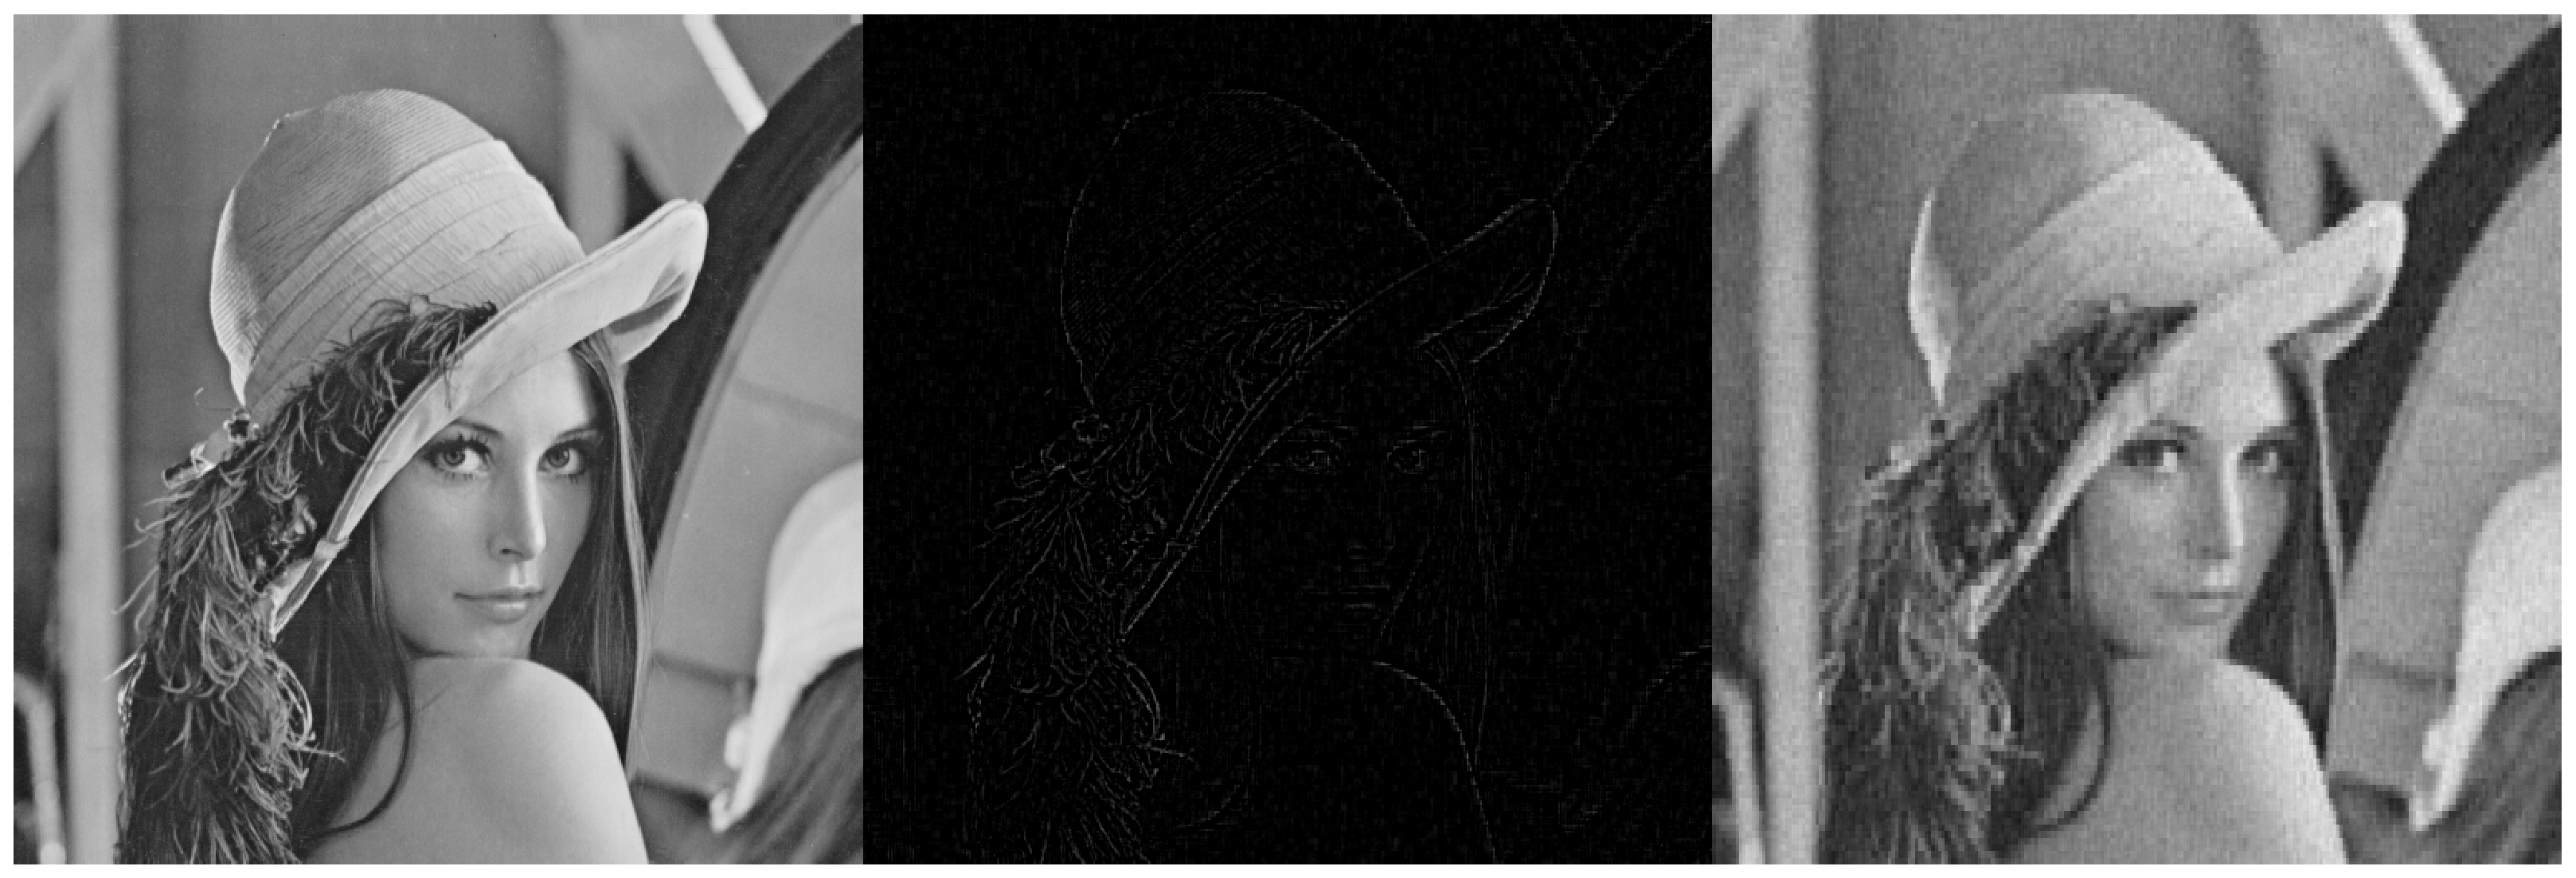
\includegraphics[width=150mm]{u01/h_out.eps}


\paragraph{Fourier}
Hier verh\"alt sich der Verlust mit blossem Auge \"ahnlich zur Hadamard Transformation. Im diesem Beispiel
wurden 255281/262144 Elemente auf $0$ gesetzt.
\\

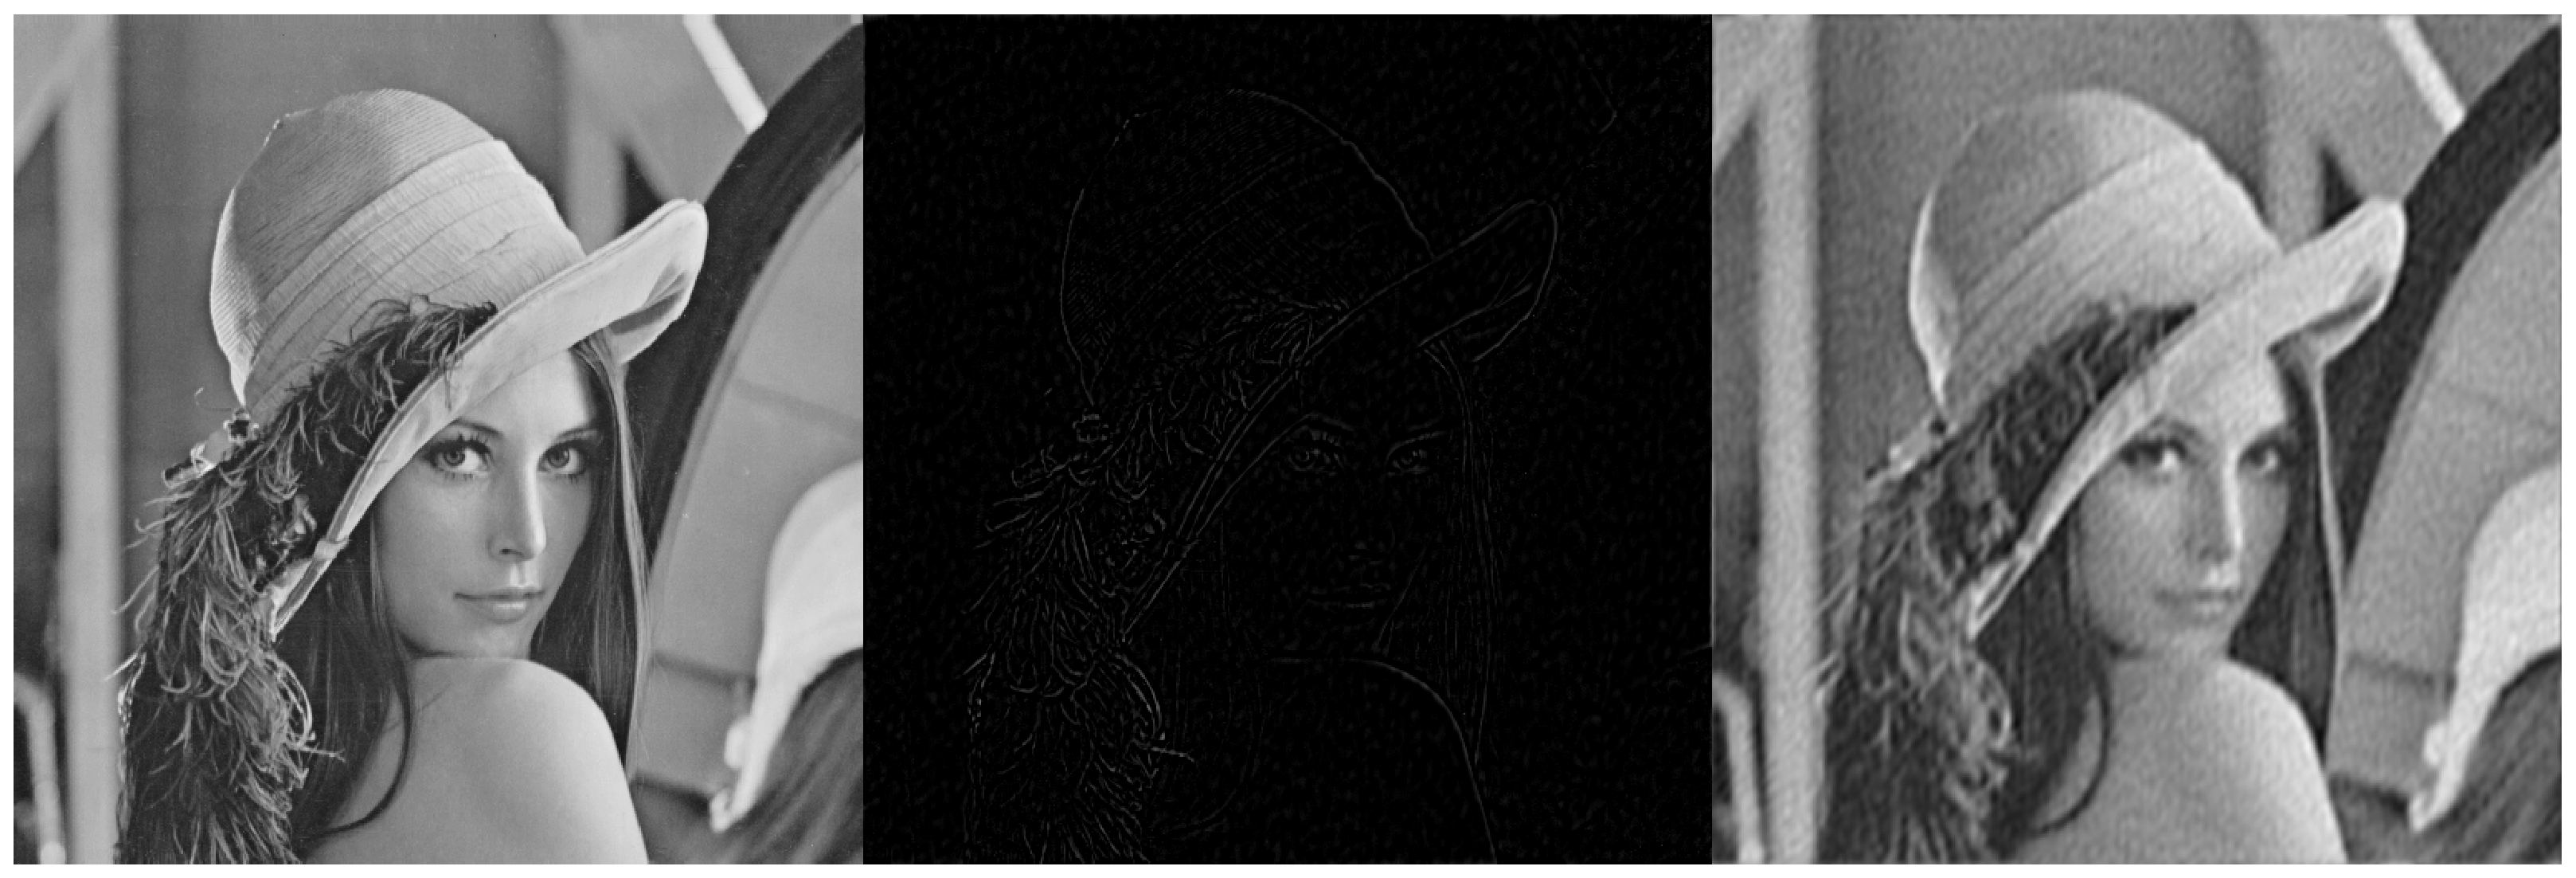
\includegraphics[width=150mm]{u01/f_out.eps}
\end{document}
